%% \teaser{
%%   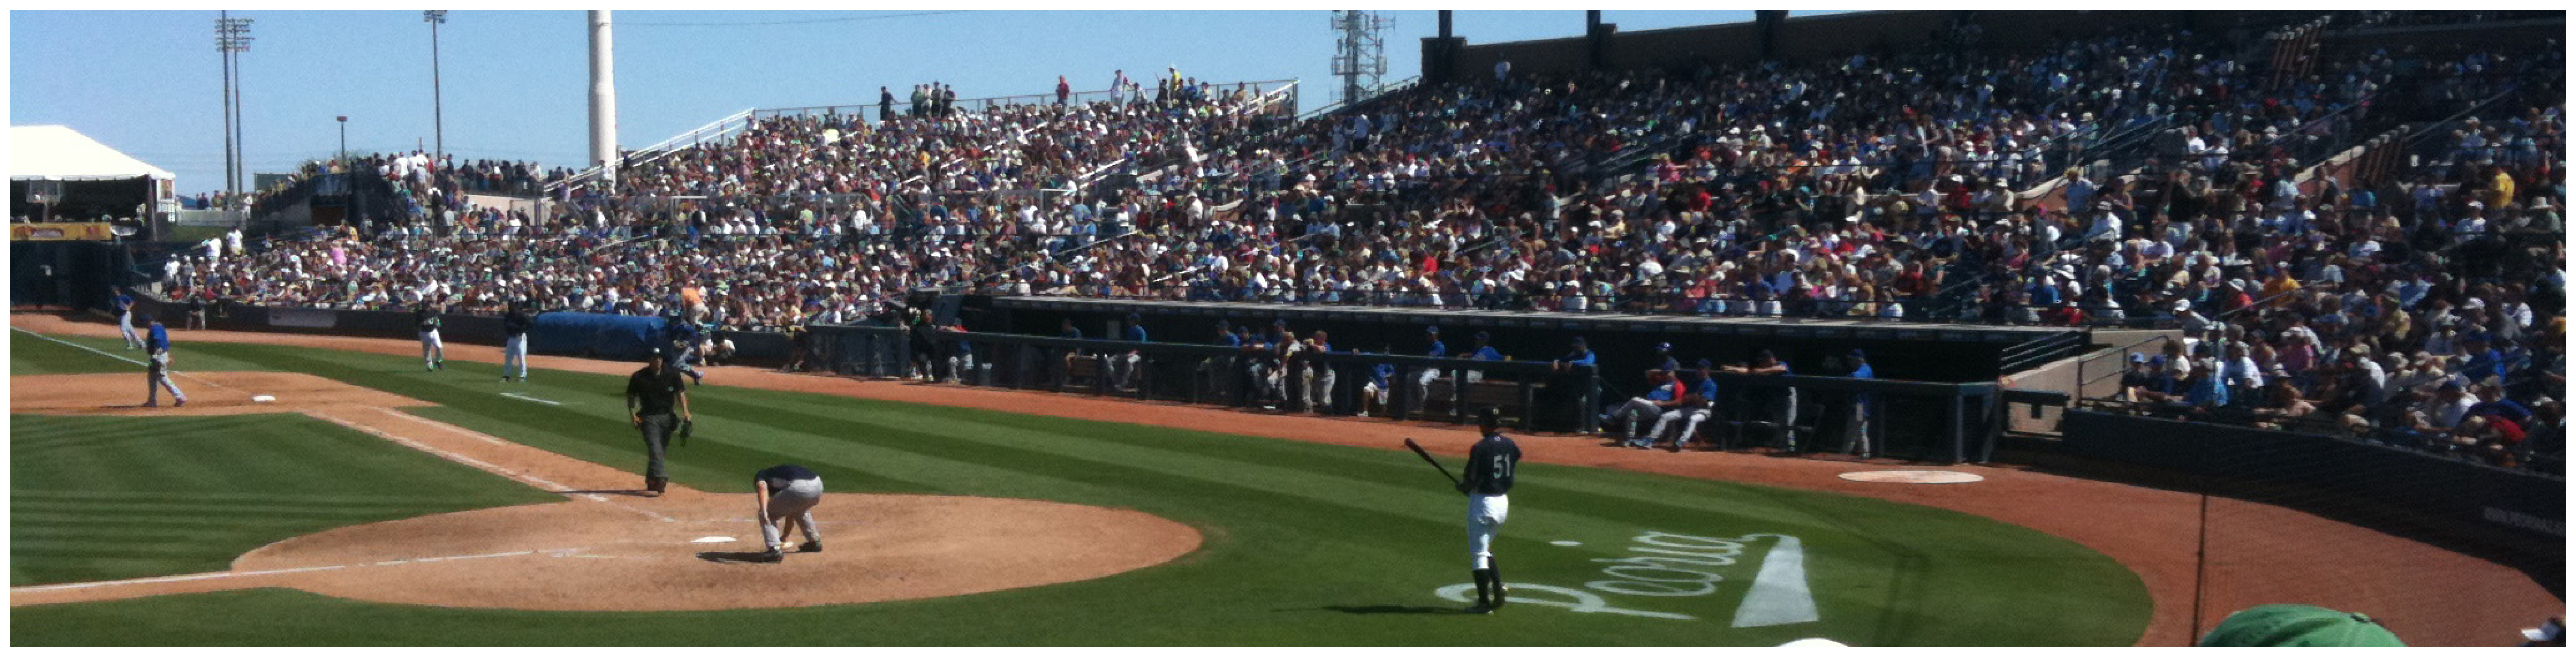
\includegraphics[height=1.5in]{images/sampleteaser}
%%   \caption{Spring Training 2009, Peoria, AZ.}
%% }

\maketitle

\begin{abstract}

Almost no method has been established that properly render compound eyes including pseudopupil, which is a characteristic optical phenomenon.
 Pseudopupil can be observed in numerous insects and crustaceans such as butterflies, dragonflies, cicadas, squilla, lobsters etc. 
We present a simple technique for rendering compound eyes in real-time, including the optical phenomenon. Our model enables efficient simulation of effects that previous models cannot reproduce. 
The middle-level micro structure of the surface, which consists of numerous ommatidia, is automatically generated by using a programmable shader.

%% Citations can be done this way~\cite{Jobs95} or this more concise 
%% way~\shortcite{Jobs95}, depending upon the application.

\end{abstract}

%%%--------------------------?? choose category?
\begin{CRcatlist}
  \CRcat{I.3.3}{Computer Graphics}{Three-Dimensional Graphics and Realism}{Display Algorithms}
  \CRcat{I.3.7}{Computer Graphics}{Three-Dimensional Graphics and Realism}{Radiosity};
\end{CRcatlist}

\keywordlist

%% Use this only if you're preparing a technical paper to be published in the 
%% ACM 'Transactions on Graphics' journal.

\TOGlinkslist

%% Required for all content. 

\copyrightspace

\section{Introduction}

Accurately modeling refraction of light through cornea is essential for realistic eye-rendering.
In particular refraction at the cornea causes a large difference in appearance.
On the one hand advanced human-eye rendering algorithms are developed and succeeded in rendering photo realistic effects in real time; on the other hand, however, limited number of studies were performed which surveyed rendering optical appearance of compound eyes in detail. 
Therefore phenomena caused by the internal structure on the surface of compound eyes were insufficiently reproduced.

In order to compensate this insufficiency, we propose a method for rendering the optical phenomenon of compound eye in real-time.
In this paper we describe a method to reproduce the unique pattern which caused by the refraction of light at the lenses of ommatidia.
Our method enables the reproduction of pseudopupil, the spot pattern: some regions of the compound eye appear dark due to the absorption of light rays by the pigment cells of ommatidia which are oriented in the same direction as the observer.


\section{Related Work}

Some entomologists have been interested in the functional structure of compound eyes.
Enumerated studies were conducted by Yagi\cite{} which include an analytic description for pseudopupil.
Nagata\cite{} carried out an experiment to artificially reproduce the appearance of pseudopupil by geometrically arranging spherical lenses on a plane and a hemisphere which are regularly dotted.
Petrowitz et al.\ \cite{} determined the optical axes of ommatidia in a certain blowfly by inspecting the deep pseudopupil.

In spite of detailed studies in the field of biology, pseudopupil is unfamiliar in the fields of computer graphics and image processing.
Few studies deal with it; for example, Bachalany et al.\ \cite{} mentioned that the phenomenon influences on the motion tracking of a dragonfly from an image sequence.
Furthermore almost no study has performed the rendering process of the phenomenon. Merely outer shapes of compound eyes are replicated as 3DCG models in the field of art design.

Hence there is room for improvement in rendering method of compound eyes, we challenged to express this phenomenon in computer graphics based on explanation and experiments in the biological field.  


%% \begin{equation}
%%  \sum_{j=1}^{z} j = \frac{z(z+1)}{2}
%% \end{equation}

%% \begin{eqnarray}
%% x & \ll & y_{1} + \cdots + y_{n} \\
%%   & \leq & z
%% \end{eqnarray}

%% \section{Exposition}

\begin{figure}[ht]
  \centering
  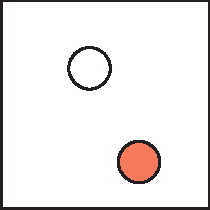
\includegraphics[width=1.5in]{images/samplefigure}
  \caption{Sample illustration.}
\end{figure}

\section{Our Method}

The main purpose of this method is to render pseudopupil pattern from polygon model that can be handled in real-time using a programmable shader. Therefore it is inefficient to create an elaborate high polygon model.
The goal is automatically generating an inner surface structure from the contour surface of the compo und eye. 

Our method applied this algorithm as a shader program to an arbitrary curved surface.
The application program inputs a texture image and basic geometry data such as positions, texture coordinates, normals to the shader program.
Paths of light are physically computed on GPU by calculating vectors from these values.

The lens of an ommatidium is treated as a sphere in order to simplify the calculation.
A sphere can be represented by simple parameters; the radius and the position of the center, which reduce the variables required for calculations.
Nagata\cite{} revealed that it is possible to sufficiently reproduce the property of pseudopupil, even if the lenses of ommatidia are approximated as spheres.

The shader process consists of roughly three stages.
The first stage is to estimate the sphere that crosses the line of sight from among the spherical lenses which are virtually set.
On the second stage, refraction calculation of incident vector is performed. Finally, UV coordinates are recalculated from the intersection of the sight path and the virtual texture plane. Then the color of the pixel is determined from the updated data.

\subsection{Incident Sphere Estimation}

For simplification, the spheres are arranged in a grid: although this arrangement is unnatural, it is sufficient to evaluate the effectiveness of this method.
The center coordinates of spheres are determined from the UV coordinates, in other words, they are determined from the three-dimensional vectors obtained by projecting the unit vectors of U-V-axes into the space.
The projected unit vectors of U-V-axes are defined as below.

%% \begin{equation}
%%  \sum_{j=1}^{z} j = \frac{z(z+1)}{2}
%% \end{equation}

%% \begin{equation}
%%  \sum_{j=1}^{z} j = \frac{z(z+1)}{2}
%% \end{equation}

%% \begin{equation}
%%  \sum_{j=1}^{z} j = \frac{z(z+1)}{2}
%% \end{equation}

Input texture coordinates of three vertices, which form the triangle polygon, are defined like$(u_0,v_0)$.
The vector values $p_0, p_1, p_2$ mean positions of vertices.
The difference between two values is expressed like,
%% \begin{equation}
%%  \sum_{j=1}^{z} j = \frac{z(z+1)}{2}
%% \end{equation}

Estimation with the intersection of the incident vector and the polygon cannot select the exact sphere that crosses the line of sight.
Therefore the intersection of the incident vector and translated plane is repeatedly calculated in order to estimate more accurate sphere\ref{}.
The plane is translated in the normal direction at regular intervals. Then the correct sphere is determined by performing intersection determination of the line of sight and the sphere.
\begin{figure}[ht]
  \centering
  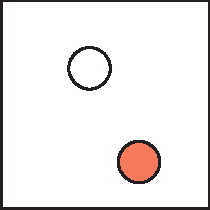
\includegraphics[width=1.5in]{images/samplefigure}
  \caption{Sample illustration.}
\end{figure}

\subsection{Refraction Calculation}
In this stage, the path of light passing through ommatidia is determined.
The inter section of sight vector and the sphere is calculated.
Then the refraction vector is calculated based on Snell’s law.
Since refracted light crosses the sphere again, the refraction vector is calculated which emerging from the sphere after determining the second intersection point.
The intersection determination with neighboring spheres is conducted and this refraction process is repeated if necessary.

\subsection{Recalculation of Texture Coordinates}
After sufficiently conducted the refraction stage, UV coordinates are recalculated from the intersection of the light path and the texture surface in \ref{}.
This intersection point will projected onto the original polygon surface.
Then recalculation of texture coordinates will be performed at the last position, which is on the polygon surface.
More precisely, the point is represented with U and V; the coefficients of them coincide with the texture coordinates of the point.
Then these values are passed to the shader as updated texture coordinates.

\section{Result and Discussion}

Rendering results of compound eye models are depicted in \ref{}.
\begin{figure}[ht]
  \centering
  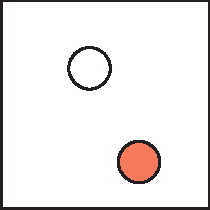
\includegraphics[width=1.5in]{images/samplefigure}
  \caption{Sample illustration.}
\end{figure}
Modeled after the experiment of Nagata, refractive index is set to 1.491 which equals to that of glass.
Radius of sphere is determined by the user and the value should be able to cover entire surface; i.e. spheres should be arranged without intervals.
The simulation runs at over 60 fps on NVIDIA GeForce GTX 660.
The largest number of polygons we used is about 18k. These performances show that our method can efficiently render the microfacet surface.

Comparison image with real photos is displayed in \ref{}.
It can be observed that the central pupil or a clearly conspicuous black spot at the center and the side pupil or the spots around the central pupil are reproduced.
The result qualitatively expresses the characteristic appearance of compound eye.

\section{Conclusion}

In this article we have presented a technique for reproducing pseudopupil pattern in real-time.
Our method can be applied to convex surfaces and smoothly depicted black spot pattern on them.
However the pattern does not naturally connected in a certain area because center positions of sphere lenses depend on the texture coordinates.
Therefore another algorithm is needed to precisely determine the positions of spheres.
We are considering a method that is independent of texture information and that directly generates positions of spheres from geometry information.


\section*{Acknowledgements}

To Robert, for all the bagels.
